\documentclass[tikz,border=8pt]{standalone}
\usepackage{amsmath}
\usepackage{pgfplots}
\usepackage{xcolor}
\pgfplotsset{compat=1.18}

\definecolor{lineblue}{HTML}{2F6DB2}
\definecolor{linegray}{HTML}{555555}

\begin{document}
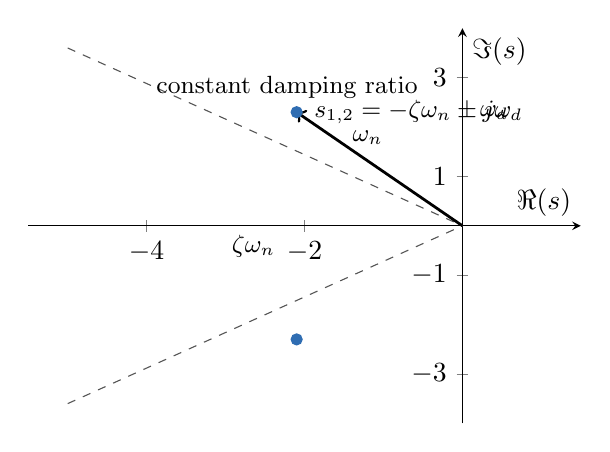
\begin{tikzpicture}
  \begin{axis}[
    width=8.6cm,
    height=6.6cm,
    xmin=-5.5, xmax=1.5,
    ymin=-4.0, ymax=4.0,
    axis lines=middle,
    xlabel={$\Re(s)$},
    ylabel={$\Im(s)$},
    xtick={-4,-2,0},
    ytick={-3,-1,1,3},
    clip=false
  ]
    \addplot[dashed, color=linegray] coordinates {(-5.0,3.6) (0,0)};
    \addplot[dashed, color=linegray] coordinates {(-5.0,-3.6) (0,0)};
    \addplot[color=lineblue, mark=*, only marks, mark size=2pt] coordinates {(-2.1,2.3) (-2.1,-2.3)};
    \node[font=\small, anchor=west] at (axis cs:-2.0,2.3) {$s_{1,2}=-\zeta\omega_n\pm j\omega_d$};
    \node[font=\small, anchor=west] at (axis cs:-4.0,2.8) {constant damping ratio};
    \draw[->, line width=1.0pt] (axis cs:0,0) -- (axis cs:-2.1,2.3);
    \node[font=\small, anchor=south] at (axis cs:-1.2,1.45) {$\omega_n$};
    \node[font=\small, anchor=north east] at (axis cs:-2.25,0.0) {$\zeta\omega_n$};
    \node[font=\small, anchor=west] at (axis cs:0.1,2.3) {$\omega_d$};
  \end{axis}
\end{tikzpicture}
\end{document}
